\documentclass[12pt,letterpaper,english]{article}
\usepackage[T1]{fontenc}
\usepackage[latin9]{inputenc}
\pagestyle{empty}
\usepackage{amsmath}
\usepackage{amssymb}
\usepackage{graphicx}
\usepackage{bm}
\usepackage{multicol}
\usepackage{enumitem}

\usepackage{hyperref}
\hypersetup{
    colorlinks=true,
    linkcolor=blue,
    filecolor=magenta,      
    urlcolor=cyan,
}

\newcommand{\norm}[1]{\lVert#1\rVert}

\makeatletter

\special{papersize=\the\paperwidth,\the\paperheight}



\textwidth6.5in\textheight9in\topmargin-.25in\oddsidemargin0in\evensidemargin0in\parskip5pt\parindent0pt


\usepackage{fancyhdr}
\pagestyle{fancy}
\lhead{Reconfigurable Mechanical Vibrations Laboratory Kit}
\rhead{}


\usepackage{lastpage}
 
 
\rfoot{Page \thepage \hspace{1pt} of \pageref{LastPage}}

%\rfoot{\small }
\lfoot{Mechanical Vibrations: Lab 2}
\cfoot{}




\usepackage{babel}


\makeatother

\usepackage{babel}
\begin{document}
\global\long\def\Re{{\rm {Re }}}
 \global\long\def\cL{{\cal L}}
 \global\long\def\sq{{\rm {sq}}}
 \global\long\def\bfx{{\bf x}}
 \global\long\def\bfi{{\bf i}}
 \global\long\def\bfj{{\bf j}}


\begin{center}
\textbf{\large Lab Assignment 2: Passive Isolation}
\par\end{center}{\large \par}


Read through section E2 in the Assembly Guide for instructions on what to assemble for this lab. 

First, add about 15 dried beans to the upper platform as shown below.
%
\begin{center}
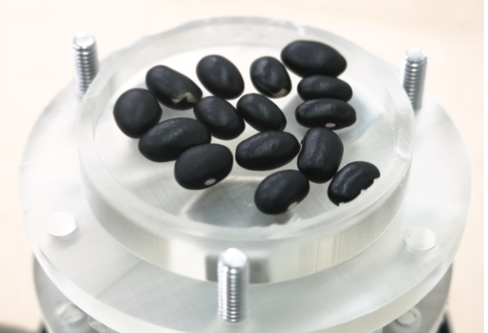
\includegraphics[width=2.5in]{lab2b.png}
\end{center}


For this lab, we will explore the effectiveness of a simple passive isolation system. The first configuration (1) contains the upper platform on the passive isolation platform {\it(with the bolts fixed}, shown in the left image below). The second configuration (2) contains the cup placed on the passive isolation rig {\it(without the bolts} so that the springs are free, as in the right image below).

\begin{center}
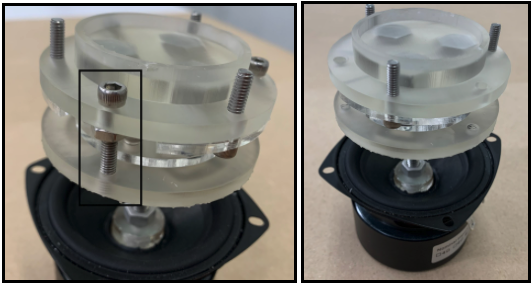
\includegraphics[width=5in]{lab2c.png}
\end{center}

Set the diving frequency to 120Hz. Note that for the entirety of this demo, the strobing is not needed (but can be experimented with if you would like). Once the shaker starts vibrating, explore configuration (1): rigid support.  Take note of the amplitude at which the beans just begin to move around on the platform. If the amplitude doesn't seem to be high enough, slowly increase the driving amplitude of the speaker until the beans clearly move.  \\

\begin{enumerate}

\item Explore how the intensity of the movement of the beans changes between configuration (1) and (2) under the same driving parameters at 120 Hz.  Take a video of the bean motion for both configurations. 
\item Repeat the above, but this time reducing the driving frequency in 20 Hz steps down to 30 Hz (and resetting the driving amplitude as needed).  
At each frequency, specifically take note as to whether the bean motion appears to be reduced, increased, or stay the same by the inclusion of the springs in configuration (2).  Explain and rationalize your observations.
\begin{itemize}
\item {\small In addition to the bean test, you can also try a ``touch'' test where you gently place your finger on the base and then on the isolation platform.  At each frequency, note how much vibration is transmitted from the base to the isolation platform.}

\end{itemize}

\item Provide feedback or ideas (positive and/or areas for improvement) on the setup process and passive isolation demonstration. 





\end{enumerate}




\end{document}
